% REV-ECIT 2026: IEEE conference format, A4 paper, maximum six pages.
% Compile with: latexmk -pdf main.tex
\documentclass[conference,a4paper]{IEEEtran}

\usepackage{iftex}
\ifPDFTeX
  \usepackage[utf8]{vietnam}
  \usepackage{textcomp}
\else
  \usepackage{fontspec}
  \defaultfontfeatures{Ligatures=TeX}
  \IfFontExistsTF{Times New Roman}{\setmainfont{Times New Roman}}{\setmainfont{TeX Gyre Termes}}
\fi
\usepackage{amsmath,amssymb}
\usepackage{booktabs,array,tabularx,makecell}
\usepackage{microtype}
\usepackage{fancyhdr}
\usepackage[table]{xcolor}
\usepackage{tikz}
\usetikzlibrary{arrows.meta,positioning,fit,backgrounds}
\usepackage{xurl}
\usepackage[unicode,hidelinks]{hyperref}
\hypersetup{
  pdftitle={Học tương phản có giám sát phân cấp ở mức token kết hợp CRF cho nhận dạng thực thể trong văn bản thủ tục hành chính tiếng Việt},
  pdfauthor={Nguyễn Thị Bích Nguyên và cộng sự},
  pdfkeywords={nhận diện thực thể, tiếng Việt, thủ tục hành chính, PAP-NER, CRF}}
\urlstyle{same}
\setlength{\emergencystretch}{2em}
\renewcommand{\arraystretch}{1.08}
\definecolor{tablehead}{RGB}{226,236,245}
\definecolor{methodrow}{RGB}{239,246,251}
\definecolor{accentblue}{RGB}{48,92,126}
\definecolor{accentorange}{RGB}{181,101,29}
\renewcommand\theadfont{\bfseries\scriptsize}
\renewcommand{\abstractname}{Tóm tắt}
\renewcommand{\IEEEkeywordsname}{Từ khóa}
\renewcommand{\refname}{Tài liệu tham khảo}

\title{Học tương phản có giám sát phân cấp ở mức token kết hợp CRF cho nhận dạng thực thể trong văn bản thủ tục hành chính tiếng Việt}
\author{
\IEEEauthorblockN{Nguyễn Thị Bích Nguyên, Lê Trung Kiên, Huỳnh Tiến Đạt \\
Đặng Thành Tài, Nguyễn Trường Giang và Nguyễn Thành Hưng}
\IEEEauthorblockA{Khoa Công nghệ Thông tin 2, Học viện Công nghệ Bưu chính Viễn thông, Việt Nam\\
Email tác giả liên hệ: \href{mailto:ntbichnguyen@ptithcm.edu.vn}{ntbichnguyen@ptithcm.edu.vn}}
}

\begin{document}
\pagestyle{fancy}
\fancyhf{}
\fancyfoot[C]{\thepage}
\renewcommand{\headrulewidth}{0pt}
\renewcommand{\footrulewidth}{0pt}
\maketitle
\thispagestyle{fancy}

\renewcommand{\abstractname}{Tóm tắt}
\begin{abstract}
Nhận diện thực thể trong văn bản thủ tục hành chính tiếng Việt gặp hai
khó khăn liên quan: thực thể dài dễ sai ranh giới và các loại ít xuất
hiện cung cấp ít mẫu dương trong mỗi mini-batch. Học tương phản theo nhãn
BIO chính xác còn tạo xung đột khi coi \texttt{B-X} và \texttt{I-X} của
cùng loại thực thể là cặp âm. Nghiên cứu này đề xuất hàm mất mát học
tương phản có giám sát phân cấp (H-SupCon): các token trùng nhãn BIO là
mẫu dương mạnh, token cùng loại nhưng khác tiền tố BIO là mẫu dương mềm,
còn nhãn \texttt{O} bị loại khỏi nhánh tương phản. H-SupCon được tối ưu
đồng thời với log-hợp lý âm của CRF; đầu chiếu chỉ dùng khi huấn luyện nên
không làm tăng đường suy luận. Trên 10.278 mẫu PAP\_NER, XLM-R +
CRF-H-SupCon và PhoBERT V2 + CRF-H-SupCon lần lượt đạt 97,28\% và
97,92\% Strict Micro F1; ELECTRA + CRF-H-SupCon đạt 98,40\%, còn đối
chứng PhoBERT V2 + CRF đạt 97,98\%. BamiBERT + CRF-H-SupCon đạt
98,48\% trên 5.162 mẫu. H-SupCon thấp hơn
đối chứng PhoBERT ghép cặp 0,06 điểm; cùng với khác biệt tập kiểm thử và
việc mỗi cấu hình mới có một lần chạy, kết quả chưa chứng minh tác động
nhân quả của loss mới. Bài viết trình bày công thức loss, kiến trúc tối ưu
chung và giao thức kiểm chứng cần thiết.
\end{abstract}

\begin{IEEEkeywords}
nhận diện thực thể, tiếng Việt, PAP\_NER, CRF, học tương phản có giám sát, ranh giới thực thể.
\end{IEEEkeywords}

\section{Giới thiệu}\label{sec:introduction}

Văn bản thủ tục hành chính thường chứa tên cơ quan thực hiện, đối tượng
áp dụng, thời điểm, số lượng và căn cứ pháp lý. Một hệ thống NER có thể
chuyển các đoạn văn bản này thành các thực thể có ranh giới và loại xác
định, phục vụ tìm kiếm, đối chiếu quy định và hỗ trợ xử lý hồ sơ. Khó
khăn nổi bật là các cụm tên cơ quan hoặc trích dẫn văn bản pháp luật có
thể dài, chứa ký hiệu và dễ bị tách sai ranh giới.

PAP\_NER là bộ dữ liệu công khai gồm năm loại thực thể: cơ quan (CQ),
đối tượng (ĐT), văn bản pháp luật (VBPL), ngày tháng (NG) và số lượng
(SL)~\cite{la2026papner}. Trong tập huấn luyện địa phương, số token
\texttt{I-VBPL} gấp khoảng 3,31 lần \texttt{B-VBPL}; đồng thời SL chỉ
chiếm 7,15\% tổng số thực thể của toàn bộ dữ liệu. Hai đặc điểm này gợi
ra một khoảng trống: mục tiêu học biểu diễn cần bảo toàn quan hệ giữa
phần mở đầu và phần thân của thực thể dài, nhưng vẫn phải giữ thông tin
ranh giới BIO và cung cấp tín hiệu đủ mạnh cho lớp hiếm.

SupCon theo nhãn BIO chính xác kéo các token cùng \texttt{B-X} hoặc cùng
\texttt{I-X} lại gần nhau, nhưng xem \texttt{B-X} và \texttt{I-X} là
cặp âm dù chúng cùng loại thực thể. Ngược lại, nếu gộp hoàn toàn hai
tiền tố thì biểu diễn có thể mất tín hiệu vị trí cần cho giải mã chuỗi.
Khoảng trống khoa học của bài toán là thiết kế quan hệ dương có mức độ,
thay vì lựa chọn nhị phân ``trùng nhãn'' hoặc ``trùng loại''.

Nghiên cứu này có ba đóng góp chính:
\begin{itemize}
    \item \textbf{Thứ nhất:} Đề xuất ma trận tương đồng phân cấp, trong đó cặp trùng BIO có trọng số 1 và cặp cùng loại khác tiền tố có trọng số $\alpha$, đồng thời loại nhãn \texttt{O} khỏi loss tương phản.

    \item \textbf{Thứ hai:} Kết hợp đồng thời H-SupCon với CRF để tối ưu cả hình học biểu diễn token và tính hợp lệ toàn cục của chuỗi nhãn; nhánh tương phản được tách khỏi suy luận.

    \item \textbf{Thứ ba:} Phân tích tín hiệu thực nghiệm theo từng loại thực thể và xác định các ablation còn thiếu để phân biệt lợi ích của H-SupCon với thay đổi cấu hình khác.
\end{itemize}

\section{Công trình liên quan}\label{sec:related-work}

PAP\_NER do La và cộng sự công bố là bộ dữ liệu nhận diện thực thể
cho văn bản thủ tục hành chính tiếng Việt, gồm 162.801 câu và
205.807 thực thể thuộc năm loại: cơ quan, đối tượng, văn bản pháp luật,
ngày tháng và số lượng~\cite{la2026papner}. Công trình này đã đánh giá BiLSTM+CRF,
ELECTRA, XLM-R, PhoBERT và PhoBERT+CRF; trong đó PhoBERT+CRF đạt
97,95\% Micro F1 trên tập kiểm thử của tác giả~\cite{la2026papner}. Đây là cơ sở
đối chiếu trực tiếp cho nghiên cứu của chúng tôi.

Các bộ dữ liệu NER tiếng Việt trước đó chủ yếu tập trung vào những
miền và loại thực thể khác. Chẳng hạn, PhoNER\_COVID19 được xây dựng
cho thông tin y tế liên quan đến COVID-19~\cite{truong2021phonercovid19}. Trong miền pháp luật
Việt Nam, Nguyen và cộng sự nghiên cứu việc trích xuất tham chiếu
và quan hệ giữa các tham chiếu trong văn bản pháp luật~\cite{nguyen2023legalreferences}. Những
công trình này cho thấy nhu cầu xử lý thực thể và cấu trúc thông tin
đặc thù theo miền, song khác PAP\_NER về tác vụ, hệ thống nhãn hoặc
dữ liệu đánh giá.

Về kiến trúc, XLM-R là mô hình tiền huấn luyện đa ngôn ngữ~\cite{conneau2020xlmr},
trong khi PhoBERT và BamiBERT được phát triển cho tiếng Việt
~\cite{nguyen2020phobert,nguyen2026bamibert}; ELECTRA sử dụng mục tiêu phân biệt token bị thay thế khi
tiền huấn luyện~\cite{clark2020electra}. Đối với gán nhãn chuỗi, CRF mô hình hóa sự phụ
thuộc giữa các nhãn liên tiếp~\cite{lafferty2001crf}. Học tương phản có
giám sát tổ chức không gian biểu diễn bằng quan hệ dương và âm
~\cite{khosla2020supcon}. CONTaiNER học khoảng cách giữa token trong NER
ít mẫu~\cite{das2022container}, còn SCL-RAI đối chiếu biểu diễn ở mức
span~\cite{si2022sclrai}. BANER cho thấy loss nhận biết ranh giới là một
hướng riêng quan trọng~\cite{guo2025baner}. Tuy vậy, các công trình này
không giải quyết trực tiếp quan hệ phân cấp giữa \texttt{B-X} và
\texttt{I-X} trong NER thủ tục hành chính đầy đủ dữ liệu, cũng chưa kết
hợp quan hệ dương mềm này với CRF trong một mục tiêu chung.

Ở NER đa phương thức, CUA-MNER kết hợp CRF và học tương phản có giám sát
ở mức token trong một mục tiêu end-to-end~\cite{yang2026cuamner}. Thiết kế
này cho thấy khả năng phối hợp tín hiệu phân biệt biểu diễn với ràng buộc
gán nhãn chuỗi, nhưng không trực tiếp so sánh với quy trình huấn luyện hai
giai đoạn. Vì vậy, lựa chọn giữa tối ưu tuần tự và tối ưu đồng thời vẫn là
một câu hỏi phương pháp luận cần kiểm chứng riêng trong bối cảnh PAP\_NER.

\section{Dữ liệu và phương pháp}\label{sec:method}

\subsection{Bộ ngữ liệu đối chuẩn PAP\_NER}\label{subsec:data}

PAP\_NER là bộ ngữ liệu đối chuẩn quy mô lớn đầu tiên cho NER trong thủ
tục hành chính tiếng Việt, được công bố trên \textit{PLOS ONE} năm
2026~\cite{la2026papner}. Ngữ liệu gồm các câu thuộc mô tả thủ tục
hành chính được công bố trên Cổng Dịch vụ công Quốc gia và các cơ sở
dữ liệu hành chính cấp tỉnh~\cite{la2026papner,la2025papnerdata}. Nội dung bao gồm tên cơ quan giải
quyết, đối tượng thực hiện thủ tục, căn cứ pháp lý, thời hạn xử lý và
các khoản phí hoặc số lượng liên quan. Văn bản đã được tách từ; những
tiếng tạo thành một từ được nối bằng dấu gạch dưới, chẳng hạn
\texttt{làm\_việc}.

Mỗi câu được lưu thành một dãy token, mỗi token nằm trên một dòng.
Trong các tệp sử dụng ở nghiên cứu này, một dòng gồm năm cột: token,
nhãn từ loại, nhãn cụm từ, nhãn thực thể và một cột phụ. Các câu được
ngăn cách bằng dòng trống. Bài toán nhận diện thực thể sử dụng chuỗi
token làm đầu vào và nhãn thực thể làm đầu ra. Ví dụ, một đoạn trong
dữ liệu có dạng:

\begin{verbatim}
05        M  I-NP  B-NG  O
ngày      N  I-NP  I-NG  O
làm_việc  V  B-VP  O     O
\end{verbatim}

Nhãn thực thể tuân theo quy ước BIO: \texttt{B-X} đánh dấu token đầu
tiên của một thực thể loại \texttt{X}, \texttt{I-X} đánh dấu các token
tiếp theo trong cùng thực thể và \texttt{O} biểu thị token không thuộc
thực thể nào. Có năm loại thực thể: CQ (cơ quan), ĐT (đối tượng), VBPL
(văn bản pháp luật), NG (ngày hoặc khoảng thời gian) và SL (số lượng).
Như vậy, bài toán sử dụng 11 nhãn ở mức token, gồm \texttt{O} và hai
nhãn \texttt{B}/\texttt{I} cho mỗi loại thực thể.

Trong các thí nghiệm được báo cáo, PAP\_NER được chia theo tỷ lệ
70/15/15, gồm 24.089 câu huấn luyện, 5.162 câu phát triển và 5.162 câu
kiểm thử. Toàn bộ thiết lập có 34.413 câu, 783.777 token và 42.489 lượt
xuất hiện thực thể. Bảng~\ref{tab:entity-distribution} trình bày số thực
thể của từng loại.

\begin{table}[t]
\centering
\caption{Phân bố thực thể trong dữ liệu thực nghiệm.}
\label{tab:entity-distribution}
\footnotesize
\setlength{\tabcolsep}{4pt}
\begin{tabularx}{\columnwidth}{@{}>{\raggedright\arraybackslash}Xr@{}}
\toprule
\thead[l]{Loại thực thể} & \thead[r]{Số lượng} \\
\midrule
CQ (cơ quan)          & 13.939 \\
ĐT (đối tượng)        & 15.218 \\
VBPL (văn bản pháp luật) & 3.968 \\
NG (ngày, thời gian)  & 8.029 \\
SL (số lượng)         & 1.335 \\
\midrule
\textbf{Tổng}         & \textbf{42.489} \\
\bottomrule
\end{tabularx}
\end{table}

\subsection{Mô hình và cấu hình thực nghiệm}\label{subsec:models}

Nghiên cứu khảo sát XLM-R Base ($\sim$270 triệu tham số), PhoBERT Base
V2 ($\sim$135 triệu), ELECTRA tiếng Việt ($\sim$110--134 triệu) và
BamiBERT ($\sim$103 triệu). XLM-R là mô hình đa ngôn ngữ; ba nhóm còn
lại hướng tới tiếng Việt~\cite{conneau2020xlmr,nguyen2020phobert,
clark2020electra,nguyen2026bamibert}. Các con số chỉ mô tả mô hình nền,
chưa gồm tầng phân loại, CRF và đầu chiếu tương phản.

Các mô hình được ghép với CRF và nhánh H-SupCon, sau đó tối ưu đồng thời.
Thiết lập huấn luyện chung kế thừa giao thức tìm kiếm trên tập phát triển
của PAP\_NER~\cite{la2026papner}; các tham số riêng của H-SupCon được quét
theo Strict Micro F1 trên tập phát triển và khóa trước khi đánh giá kiểm thử.

\begin{table*}[t]
\centering
\scriptsize
\caption{Siêu tham số huấn luyện, không gian tìm kiếm và tiêu chí lựa chọn.}
\label{tab:training-hyperparams}
\setlength{\tabcolsep}{3pt}
\renewcommand{\arraystretch}{1.06}
\begin{tabularx}{\textwidth}{@{}>{\raggedright\arraybackslash}p{3.0cm}
>{\raggedright\arraybackslash}p{2.35cm}
>{\raggedright\arraybackslash}p{5.1cm}
>{\raggedright\arraybackslash}X@{}}
\toprule
\thead[l]{Siêu tham số} & \thead[l]{Giá trị chọn} &
\thead[l]{Không gian tìm kiếm} & \thead[l]{Tiêu chí lựa chọn} \\
\midrule
Optimizer & AdamW & \{Adam, AdamW, SGD\} & Strict Micro F1 trên tập phát triển \\
Tốc độ học encoder & $2\!\times\!10^{-5}$ &
$\{1\!\times\!10^{-5},2\!\times\!10^{-5},5\!\times\!10^{-5}\}$ & Hội tụ ổn định \\
Tốc độ học CRF và đầu chiếu & $1\!\times\!10^{-3}$ &
$\{5\!\times\!10^{-4},1\!\times\!10^{-3},2\!\times\!10^{-3}\}$ & Đầu tác vụ hội tụ nhanh \\
Lịch tốc độ học & Linear decay + warm-up & \{constant, linear, cosine\} & F1 cuối tốt nhất \\
Tỷ lệ warm-up & 0,1 & \{0,05; 0,1; 0,2\} & Giảm bất ổn đầu quá trình \\
Epoch tối đa / patience & 20 / 3 & \{10, 20, 30\} / \{2, 3, 5\} & Dừng sớm theo F1 phát triển \\
Độ dài chuỗi tối đa & 256 token & \{128, 256, 512\} & Bao phủ gần như toàn bộ câu \\
Weight decay / gradient clipping & 0,01 / 1,0 &
\{0,001; 0,01; 0,1\} / \{0,5; 1,0; 5,0\} & Điều chuẩn và ổn định gradient \\
Dropout / mixed precision & 0,1 / FP16 & \{0; 0,1; 0,2\} / \{FP32, FP16\} &
Cân bằng điều chuẩn và tốc độ; CRF tính ở FP32 \\
Batch size $B$ & 128 & \{16, 32, 128\} & Tăng số cặp dương tương phản trong batch \\
\midrule
Trọng số H-SupCon $\lambda$ & 0,3 & \{0,1; 0,2; 0,3; 0,5; 0,7\} & Strict Micro F1 phát triển lớn nhất \\
Liên kết mềm $\alpha$ & 0,3 & \{0; 0,1; 0,2; 0,3; 0,4; 0,5\} & F1 VBPL và chất lượng ranh giới \\
Nhiệt độ $\tau$ & 0,07 & \{0,05; 0,07; 0,1; 0,15\} & Phân tách mẫu âm khó ổn định \\
\bottomrule
\end{tabularx}
\end{table*}

Bảng~\ref{tab:training-hyperparams} thay cấu hình batch 32 của benchmark
PAP\_NER bằng batch 128 cho nhánh tương phản, nhằm cung cấp nhiều cặp dương
hơn trong mỗi bước cập nhật. AMP dùng FP16 cho encoder và đầu chiếu, nhưng
CRF được ép về FP32 để tránh mất ổn định số. Mọi lựa chọn chỉ dựa trên tập
phát triển; tập kiểm thử không tham gia tìm kiếm siêu tham số.

\subsection{Chiến lược tối ưu hóa: hai giai đoạn và đồng thời}\label{subsec:optimization}
Với \textit{Two-Stage}, encoder được fine-tune bằng loss tương phản trước,
sau đó huấn luyện cùng CRF; giai đoạn sau vì thế có thể ghi đè không gian
biểu diễn đã học. \textit{Joint Optimization} truyền đồng thời hai gradient
qua encoder trong mỗi mini-batch; CUA-MNER là một thiết kế token-level gần
đây theo hướng này~\cite{yang2026cuamner}. Bài báo chọn Joint theo
Phương trình~\eqref{eq:joint-loss} như một giả thuyết thiết kế. So sánh công
bằng với Two-Stage vẫn phải giữ nguyên encoder, seed và số lần cập nhật.

\subsection{Hàm mất mát đề xuất CRF--H-SupCon}\label{subsec:loss}

Cùng biểu diễn token $\mathbf h_i\in\mathbb R^d$ được đưa vào hai nhánh
huấn luyện có vai trò khác nhau.

\noindent\textbf{Mất mát CRF.} Với câu $\mathbf x$ dài $n$, gọi
$\mathbf e_i[y_i]$ là điểm phát xạ của nhãn $y_i$ và $A_{u,v}$ là điểm
chuyển từ nhãn $u$ sang $v$. Điểm và xác suất của toàn chuỗi BIO là
\begin{equation}
\begin{aligned}
S(\mathbf x,\mathbf y)
 &=\sum_{i=1}^{n}\bigl(\mathbf e_i[y_i]+A_{y_{i-1},y_i}\bigr),\\
p_{\mathrm{CRF}}(\mathbf y\mid\mathbf x)
 &=\frac{\exp S(\mathbf x,\mathbf y)}
 {\sum_{\mathbf y'\in\mathcal Y(\mathbf x)}\exp S(\mathbf x,\mathbf y')}.
\end{aligned}
\label{eq:crf-probability}
\end{equation}
Với mini-batch $\mathcal B$, CRF tối thiểu hóa log-hợp lý âm
\begin{equation}
\mathcal L_{\mathrm{CRF}}
=-\frac{1}{|\mathcal B|}\sum_{(\mathbf x,\mathbf y)\in\mathcal B}
\log p_{\mathrm{CRF}}(\mathbf y\mid\mathbf x),
\label{eq:crf-loss}
\end{equation}
qua đó học đồng thời điểm phát xạ và ràng buộc chuyển tiếp toàn chuỗi;
Viterbi được dùng để tìm chuỗi có điểm lớn nhất khi suy luận
~\cite{lafferty2001crf}.

\noindent\textbf{Mất mát tương phản phân cấp.} Đầu chiếu hai tầng tạo
$\mathbf z_i=g(\mathbf h_i)/\|g(\mathbf h_i)\|_2$. Khác SupCon chuẩn
~\cite{khosla2020supcon}, nhánh đề xuất chỉ xét token thực thể
$\mathcal I_e=\{i\mid y_i\ne\texttt{O}\}$ và phân biệt hai mức quan hệ
dương. Gọi $t(y)$ là loại thực thể sau khi bỏ tiền tố BIO. Với $i\ne j$:
\begin{equation}
w_{ij}=\begin{cases}
1, & y_i=y_j,\\
\alpha, & t(y_i)=t(y_j),\ y_i\ne y_j,\\
0, & \text{ngược lại},
\end{cases}\qquad 0<\alpha<1.
\label{eq:weights}
\end{equation}
Cặp trùng BIO là mẫu dương mạnh; cặp \texttt{B-X}/\texttt{I-X} cùng
loại là mẫu dương mềm. Cách này duy trì liên kết ngữ nghĩa trong thực
thể dài nhưng không đồng nhất hoàn toàn vai trò ranh giới. Với
$\mathcal A(i)=\mathcal I_e\setminus\{i\}$ và
$s_{ik}=\mathbf z_i^\top\mathbf z_k/\tau$, loss cho anchor hợp lệ là:
\begin{equation}
\ell_i=-\frac{1}{\sum_{j\in\mathcal A(i)}w_{ij}}
\sum_{j\in\mathcal A(i)}w_{ij}
\log\frac{e^{s_{ij}}}{\sum_{k\in\mathcal A(i)}e^{s_{ik}}}.
\label{eq:hsupcon-anchor}
\end{equation}
Đặt $\mathcal V=\{i\in\mathcal I_e\mid
\sum_{j\in\mathcal A(i)}w_{ij}>0\}$, mất mát của nhánh tương phản là
\begin{equation}
\mathcal L_{\mathrm{H\text{-}SupCon}}
=\frac{1}{|\mathcal V|}\sum_{i\in\mathcal V}\ell_i.
\label{eq:hsupcon-loss}
\end{equation}
Việc chỉ lấy trung bình trên $\mathcal V$ tránh phép chia cho 0 khi batch
không chứa cặp dương cho một anchor.

\noindent\textbf{Mục tiêu tối ưu chung.} Hai định nghĩa trên được kết hợp:
\begin{equation}
\mathcal L_{\mathrm{joint}}=\mathcal L_{\mathrm{CRF}}+
\lambda\mathcal L_{\mathrm{H\text{-}SupCon}},
\quad \lambda=0{,}3,\ \alpha=0{,}3,\ \tau=0{,}07.
\label{eq:joint-loss}
\end{equation}
Gradient từ hai số hạng được cộng tại encoder dùng chung: CRF bảo toàn
tính hợp lệ của chuỗi, còn H-SupCon kéo gần token trùng BIO với trọng số
$1$ và token cùng loại khác tiền tố với trọng số $\alpha$. Nhãn \texttt{O}
vẫn tham gia đầy đủ vào CRF nhưng không chi phối nhánh tương phản. Khi
kiểm thử, đầu chiếu bị loại; đường suy luận chỉ còn encoder, tầng phát xạ
và Viterbi, nên loss mới không làm tăng chi phí suy luận.

\begin{figure*}[t]
\centering
\begin{tikzpicture}[
  font=\footnotesize,
  block/.style={draw=accentblue, fill=tablehead, line width=0.7pt,
    rounded corners=2.5pt, align=center, minimum height=9mm, text width=21mm},
  head/.style={draw=accentorange, fill=orange!8, line width=0.7pt,
    rounded corners=2.5pt, align=center, minimum height=9mm, text width=22mm},
  output/.style={draw=black!65, fill=black!3, line width=0.7pt,
    rounded corners=2.5pt, align=center, minimum height=9mm, text width=20mm},
  objective/.style={draw=accentblue, fill=methodrow, line width=1pt,
    rounded corners=2.5pt, align=center, minimum height=10mm, text width=25mm},
  flow/.style={-{Latex[length=2.2mm]}, line width=0.8pt, draw=accentblue},
  train/.style={-{Latex[length=2.2mm]}, line width=0.8pt, draw=accentorange, dashed}
]
\node[block] (input) at (0,0) {Câu tiếng Việt\\$x_{1:n}$};
\node[block] (encoder) at (2.8,0) {Bộ mã hóa\\tiền huấn luyện};
\node[block] (repr) at (5.6,0) {Biểu diễn token\\$\mathbf h_i$};
\node[head] (emit) at (8.4,1.0) {Tầng phát xạ\\$\mathbf e_i$};
\node[block] (crf) at (11.2,1.0) {Linear-chain CRF\\$\mathcal L_{\mathrm{CRF}}$};
\node[output] (tags) at (14.0,1.0) {Viterbi\\chuỗi BIO};
\node[head] (proj) at (8.4,-1.0) {Đầu chiếu\\$d\!\to\!256\!\to\!128$};
\node[block] (supcon) at (11.2,-1.0) {H-SupCon\\$w_{ij}\!\in\!\{1,\alpha,0\}$};
\node[objective] (joint) at (14.0,-1.0) {Mục tiêu chung\\$\mathcal L_{\mathrm{CRF}}+\lambda\mathcal L_{\mathrm{H\text{-}SupCon}}$};
\draw[flow] (input) -- (encoder);
\draw[flow] (encoder) -- (repr);
\draw[flow] (repr) -- (emit);
\draw[flow] (emit) -- (crf);
\draw[flow] (crf) -- node[above, font=\scriptsize]{suy luận} (tags);
\draw[train] (repr) -- node[below left, font=\scriptsize]{chỉ huấn luyện} (proj);
\draw[train] (proj) -- (supcon);
\draw[train] (crf) -- (joint);
\draw[train] (supcon) -- (joint);
\begin{scope}[on background layer]
  \node[fit=(emit)(crf)(tags), rounded corners=4pt, fill=blue!2,
    inner sep=4pt, label={[font=\scriptsize\bfseries, text=accentblue]above:Nhánh gán nhãn chuỗi}] {};
  \node[fit=(proj)(supcon)(joint), rounded corners=4pt, fill=orange!3,
    inner sep=4pt, label={[font=\scriptsize\bfseries, text=accentorange]below:Nhánh tương phản có giám sát}] {};
\end{scope}
\end{tikzpicture}
\caption{Kiến trúc huấn luyện chung CRF--H-SupCon. Đường màu xanh biểu diễn
luồng suy luận; đường màu cam nét đứt biểu diễn các kết nối chỉ dùng khi huấn luyện.}
\label{fig:architecture}
\end{figure*}

Hình~\ref{fig:architecture} thể hiện hai tín hiệu bổ trợ: CRF học phụ
thuộc chuyển tiếp của toàn chuỗi, còn H-SupCon tổ chức hình học biểu
diễn ở mức token. Tối ưu đồng thời cho phép cả hai gradient cập nhật
encoder trong cùng một bước, tránh việc không gian tương phản bị thay
đổi ở một giai đoạn huấn luyện CRF tách biệt.

\subsection{Phép đánh giá}\label{subsec:evaluation}

Một thực thể chỉ được tính đúng khi cả ranh giới và loại đều khớp nhãn
chuẩn. Chỉ số chính là Strict Micro F1, tính từ tổng $TP$, $FP$ và $FN$
của năm loại thực thể:
\begin{align}
P_{\mathrm{micro}}
 &= \frac{\sum_c TP_c}{\sum_c(TP_c+FP_c)},\\
R_{\mathrm{micro}}
 &= \frac{\sum_c TP_c}{\sum_c(TP_c+FN_c)},\\
F_{1,\mathrm{micro}}
 &= \frac{2P_{\mathrm{micro}}R_{\mathrm{micro}}}
 {P_{\mathrm{micro}}+R_{\mathrm{micro}}}.
\end{align}
Các chỉ số theo loại và Macro F1 được báo cáo để tránh việc lớp lớn chi
phối diễn giải. Điểm được tính theo chuẩn BIO bằng
\texttt{seqeval} với \texttt{mode='strict'} và
\texttt{scheme=IOB2}~\cite{nakayama2018seqeval}.

Phân tích lỗi dùng thêm bốn chế độ: \textbf{Strict} yêu cầu đúng ranh giới
và loại; \textbf{Exact} chỉ yêu cầu đúng ranh giới; \textbf{Partial} yêu cầu
hai vùng giao nhau; \textbf{Type} yêu cầu vùng giao nhau và đúng loại.
Điểm kiểm soát được chọn theo F1 thực thể trên tập phát triển.
\section{Kết quả}\label{sec:results}

\subsection{So sánh tổng quan}\label{subsec:overall}

Kết quả so sánh cho thấy sự khác biệt về hiệu suất giữa các kiến trúc
Transformer được đánh giá, đồng thời làm rõ tác động quan sát được của việc
tích hợp học tương phản có giám sát phân cấp (\textit{Hierarchical Supervised
Contrastive Learning}, H-SupCon) vào kiến trúc gán nhãn chuỗi dựa trên CRF.

\begin{table}[t]
\centering
\footnotesize
\caption{Kết quả Strict Micro ở cấp thực thể trên PAP\_NER (\%).}
\label{tab:overall-f1}
\setlength{\tabcolsep}{2pt}
\begin{tabular*}{\columnwidth}{@{\extracolsep{\fill}}lccc@{}}
\toprule
\thead[l]{Mô hình} & \thead{P} & \thead{R} & \thead{F1} \\
\midrule
XLM-R + CRF-H-SupCon & 97,89 & 96,67 & 97,28 \\
PhoBERT V2 + CRF & 98,75 & 97,22 & 97,98 \\
PhoBERT V2 + CRF-H-SupCon & 98,65 & 97,21 & 97,92 \\
ELECTRA + CRF-H-SupCon & 98,20 & 98,60 & 98,40 \\
BamiBERT + CRF-H-SupCon & 98,03 & 98,93 & 98,48 \\
\bottomrule
\end{tabular*}
\end{table}

\noindent\textbf{Hiệu suất giữa các mô hình Transformer nền tảng
(Performance Across Transformer Backbones).} Khi được đánh giá trên cùng tập
kiểm thử gồm 10.278 mẫu, PhoBERT V2 + CRF-H-SupCon đạt cao hơn XLM-R +
CRF-H-SupCon lần lượt 0,76; 0,54 và 0,64 điểm phần trăm về Precision, Recall
và F1-score. Sự cải thiện nhất quán này gợi ý lợi thế tiềm năng của mô hình
tiền huấn luyện chuyên biệt cho tiếng Việt so với biểu diễn đa ngôn ngữ trong
NER văn bản hành chính. Nói cách khác, biểu diễn ngữ cảnh đơn ngữ có thể nắm
bắt tốt hơn các đặc trưng ngôn ngữ và cách diễn đạt chuyên biệt của miền này.

\noindent\textbf{Nhận xét 2.} Với cùng backbone PhoBERT V2, CRF-H-SupCon
đạt 98,65/97,21/97,92, thấp hơn CRF lần lượt 0,10/0,01/0,06 điểm P/R/F1;
do đó lần chạy hiện tại chưa cho thấy lợi ích tổng thể của loss mới.

\noindent\textbf{Nhận xét 3.} ELECTRA đạt
98,20/98,60/98,40 về P/R/F1. BamiBERT có F1 98,48\%, cao hơn 0,08 điểm
về trị số, nhưng được đánh giá trên 5.162 mẫu nên không xếp hạng trực tiếp.

\begin{figure}[t]
\centering
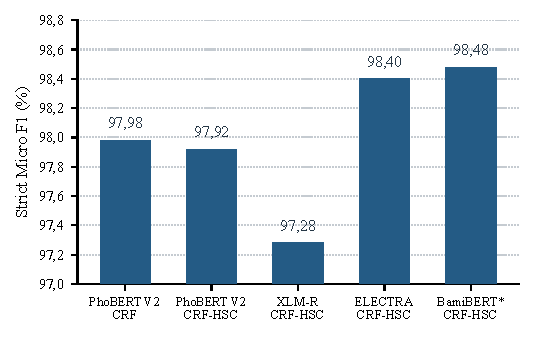
\includegraphics[width=\columnwidth]{figures/model_f1_comparison.pdf}
\caption{So sánh Strict Micro F1 của năm cấu hình mô hình. BamiBERT (*)
được đánh giá trên 5.162 mẫu nên chỉ dùng để tham khảo định tính.}
\label{fig:model-f1}
\end{figure}

\subsection{Tín hiệu thực nghiệm của H-SupCon}\label{subsec:decoders}

Theo loại thực thể trên 10.278 mẫu, chênh lệch PhoBERT V2 + CRF-H-SupCon
trừ XLM-R + CRF-H-SupCon lần
lượt là $+0{,}64$ (CQ), $+1{,}19$ (ĐT), $-0{,}10$ (VBPL), $-0{,}04$
(NG) và $+0{,}40$ điểm (SL). Kết quả cho thấy lựa chọn encoder vẫn ảnh
hưởng đáng kể đến biểu diễn được tối ưu bởi cùng mục tiêu H-SupCon.

Đối chứng PhoBERT V2 + CRF là phép so sánh cùng backbone duy nhất hiện có;
XLM-R, ELECTRA và BamiBERT vẫn thiếu đối chứng khi tắt nhánh tương phản. Kết luận
nhân quả cần giữ nguyên encoder, split, seed, batch và CRF reduction, sau
đó chỉ thay các thành phần của loss ở Phương
trình~\eqref{eq:weights}--\eqref{eq:joint-loss}.

\subsection{Phân tích theo loại thực thể}\label{subsec:entity-types}

\begin{table}[t]
\centering
\fontsize{6.6}{7.4}\selectfont
\caption{F1 theo loại thực thể (\%).}
\label{tab:entity-f1}
\setlength{\tabcolsep}{0pt}
\begin{tabular*}{\columnwidth}{@{\extracolsep{\fill}}lccccc@{}}
\toprule
\thead[l]{Mô hình} & \thead{CQ} & \thead{ĐT} & \thead{VBPL} & \thead{NG} & \thead{SL} \\
\midrule
XLM-R + CRF-H-SupCon & 97,05 & 96,02 & 97,41 & 99,99 & 96,99 \\
PhoBERT V2 + CRF & 97,74 & 97,32 & 97,41 & 99,98 & 97,24 \\
PhoBERT V2 + CRF-H-SupCon & 97,69 & 97,21 & 97,31 & 99,95 & 97,39 \\
ELECTRA + CRF-H-SupCon & 97,80 & 97,80 & 96,80 & 99,70 & 97,40 \\
BamiBERT + CRF-H-SupCon & 98,98 & 98,07 & 95,50 & 99,84 & 98,51 \\
\bottomrule
\end{tabular*}
\end{table}

Với PhoBERT V2, CRF-H-SupCon chỉ cao hơn CRF ở SL ($+0{,}15$ điểm), nhưng
thấp hơn ở CQ ($-0{,}05$), ĐT ($-0{,}11$), VBPL ($-0{,}10$) và NG
($-0{,}03$). Macro F1 tương ứng là 97,91\% và 97,94\%. ELECTRA đạt
Macro F1 97,90\%, tốt nhất ở NG (99,70\%) và thấp nhất ở VBPL (96,80\%).
BamiBERT đạt F1 thấp nhất ở VBPL (95,50\%) trong log 5.162 mẫu; kết quả không được xếp
hạng trực tiếp với các hàng dùng 10.278 mẫu. Bảng hiện chưa có khoảng tin
cậy cho các chênh lệch theo nhãn.

\subsection{Ablation cần thiết}\label{subsec:resources}

Bốn cấu hình tối thiểu cần được chạy trên cùng điều kiện: (i) CRF;
(ii) CRF + SupCon trùng BIO ($\alpha=0$); (iii) CRF + H-SupCon nhưng giữ
\texttt{O}; và (iv) CRF + H-SupCon đầy đủ. Cần quét $\alpha$, $\lambda$
và $\tau$ chỉ trên tập phát triển; báo cáo tỷ lệ anchor hợp lệ theo nhãn,
ít nhất ba seed, khoảng tin cậy và kiểm định cặp trên cùng tập kiểm thử.
Thiết kế này lần lượt kiểm chứng vai trò của liên kết mềm, việc loại
\texttt{O}, độ ổn định và ý nghĩa thống kê của mức tăng. Ngoài ra, cần
so sánh Two-Stage với Joint Optimization dưới cùng số bước cập nhật và
ngân sách tính toán để tách lợi ích của loss khỏi lịch huấn luyện.

\section{Thảo luận}\label{sec:discussion}

Trên PhoBERT V2, CRF-H-SupCon thấp hơn CRF 0,06 điểm F1 trong một lần chạy.
Khác biệt giữa XLM-R, PhoBERT V2 và ELECTRA còn phản ánh ảnh hưởng backbone;
BamiBERT chỉ có ý nghĩa mô tả do dùng tập kiểm thử khác kích thước. Về cơ
chế, CRF ràng buộc chuyển tiếp nhãn, còn H-SupCon định hình biểu diễn token;
đầu chiếu bị loại khi suy luận nên chỉ làm tăng chi phí huấn luyện.

Việc thiếu ablation $\alpha=0$, giữ/bỏ \texttt{O} và nhiều seed chưa cho
phép tách tác động của loss mới. PAP\_NER cũng chỉ đo nhận diện trích dẫn
pháp luật trong thủ tục hành chính, không đại diện cho mọi văn bản pháp lý.

\section{Hạn chế và hướng phát triển}\label{sec:limitations}

\subsection{Giá trị nội tại và độ tin cậy thống kê}

Mỗi cấu hình hiện chỉ có một lần chạy, nên chênh lệch nhỏ có thể nằm trong
dao động do seed, mini-batch và dropout. Cần chạy tối thiểu năm seed, báo cáo
trung bình, độ lệch chuẩn, khoảng tin cậy 95\% và bootstrap ghép cặp ở cấp
câu hoặc tài liệu.

Chỉ PhoBERT V2 có đối chứng CRF cùng backbone; XLM-R, ELECTRA và BamiBERT
chưa có cặp tương ứng. Ablation nhân quả phải giữ nguyên checkpoint, seed,
batch, số bước, lịch học và quy tắc chọn mô hình; so sánh Two-Stage--Joint
cũng phải dùng cùng số lần cập nhật hoặc ngân sách FLOPs.

\subsection{Giới hạn của phép đo và phân tích cơ chế}

Strict Micro F1 phù hợp với mục tiêu nhận diện chính xác cả ranh giới lẫn
loại, nhưng bị chi phối bởi các lớp phổ biến và không cho biết lỗi xuất hiện
ở vị trí nào trong thực thể. F1 theo loại ở Bảng~\ref{tab:entity-f1} mới là
bước đầu. Để kiểm tra trực tiếp giả thuyết về ranh giới dài, cần phân tầng
kết quả theo độ dài thực thể (1, 2--3, 4--7 và trên 7 token), đồng thời tách
ba nhóm lỗi: đúng vùng nhưng sai loại, đúng loại nhưng thiếu/thừa biên, và
bỏ sót hoàn toàn. Nếu H-SupCon thực sự liên kết tốt hơn \texttt{B-X} với
\texttt{I-X}, mức cải thiện phải tập trung ở nhóm thực thể nhiều token và
lỗi đứt ranh giới, thay vì chỉ tăng Micro F1 tổng.

Trọng số mềm $\alpha=0,3$ hiện được dùng như nhau cho mọi loại thực thể và
mọi độ dài. Giả định này đơn giản nhưng có thể không phù hợp khi cấu trúc
của CQ, VBPL và SL khác nhau đáng kể. Giá trị $\alpha$ quá nhỏ không bổ sung
đủ mẫu dương; giá trị quá lớn có nguy cơ làm mờ vai trò khác nhau của tiền
tố \texttt{B} và \texttt{I}. Tương tự, việc loại nhãn \texttt{O} giúp giảm
ưu thế số lượng của token ngoài thực thể, nhưng cũng bỏ qua các mẫu âm khó
ngay sát biên. Vì thế, cần báo cáo tỷ lệ anchor hợp lệ theo nhãn, số cặp
dương mạnh/mềm trong mỗi batch và phân bố cosine similarity trước và sau
huấn luyện. Các đại lượng này cho biết loss có thay đổi hình học biểu diễn
theo đúng cơ chế dự kiến hay không.

Hướng mở rộng có thể dùng $\alpha_c$ theo loại/độ dài và tăng dần $\lambda$
sau warm-up. Do loss phụ thuộc các cặp dương trong mini-batch, thí nghiệm
cần cố định danh sách batch giữa các đối chứng, ghi tỷ lệ anchor bị loại theo
lớp và so sánh lấy mẫu ngẫu nhiên, phân tầng cùng hàng đợi biểu diễn. Mọi cơ
chế thích nghi phải được chọn trên tập phát triển dưới cùng ngân sách tìm kiếm.

\subsection{Khả năng khái quát và hiệu quả tính toán}

PAP\_NER chỉ đại diện cho ngôn ngữ thủ tục hành chính. Câu văn trong văn
bản quy phạm pháp luật, bản án và hợp đồng có cấu trúc lập luận, độ dài và
hệ thống trích dẫn khác. Vì vậy, kết quả hiện tại chưa chứng minh H-SupCon
ổn định trước dịch chuyển miền. Đánh giá tương lai nên huấn luyện trên
PAP\_NER rồi kiểm thử chéo trên một tập được gán nhãn từ miền pháp lý khác;
sau đó so sánh zero-shot với fine-tune ít mẫu. Cũng cần chia kết quả theo
nguồn, thời gian ban hành và nhóm thủ tục để phát hiện trường hợp mô hình
ghi nhớ mẫu diễn đạt quen thuộc thay vì học đặc trưng ranh giới có thể
chuyển giao.

Nhánh chiếu được bỏ khi suy luận, nên kiến trúc không thêm phép tính vào
đường giải mã. Tuy nhiên, điều này không đồng nghĩa chi phí tổng bằng không:
huấn luyện vẫn phải tạo ma trận tương đồng giữa các token thực thể, với bộ
nhớ và số phép tính tăng gần bậc hai theo số anchor trong batch. Báo cáo
tiếp theo cần đo thời gian huấn luyện mỗi epoch, bộ nhớ GPU cực đại, thông
lượng câu/giây, độ trễ suy luận và kích thước mô hình trong cùng môi trường.
Nếu ma trận cặp trở thành nút thắt, có thể khảo sát lấy mẫu cặp theo lớp,
giới hạn số anchor, hàng đợi biểu diễn qua batch hoặc khai thác hard
negative cục bộ quanh biên thực thể.

Đánh giá triển khai cần đo hiệu chuẩn, khả năng từ chối và đường cong
coverage--risk vì lỗi VBPL/CQ có thể ảnh hưởng truy xuất, còn lỗi SL có thể
làm đổi điều kiện áp dụng. Một bộ kiểm thử stress giữ nguyên nhãn vàng nên
thêm có kiểm soát lỗi OCR, dấu tiếng Việt, khoảng trắng, viết tắt và chuỗi
trích dẫn; độ giảm F1 so với đối chứng phản ánh độ bền ngoài phân bố quen thuộc.

\subsection{Đánh giá ngoại sinh và cập nhật mô hình}

Giá trị ứng dụng cần được kiểm tra trên tác vụ phía sau với ba biến thể dùng
chung retriever và bộ sinh: không dùng NER, dùng thực thể dự đoán và dùng
nhãn vàng. Recall@$k$, MRR/nDCG, độ chính xác trích dẫn và tỷ lệ câu trả lời
được hỗ trợ bởi nguồn cho biết lỗi CQ/VBPL có thực sự ảnh hưởng truy xuất hay
không; mọi thành phần ngoài NER phải được cố định để tránh quy kết nhầm.

Khi triển khai, mỗi mô hình cần gắn với phiên bản dữ liệu, ontology nhãn,
ngưỡng từ chối và bộ kiểm thử hồi quy. Phiên bản mới chỉ nên thay thế mô hình
đang vận hành khi không làm giảm đáng kể F1 của lớp quan trọng và vượt qua
bộ kiểm thử stress về OCR, dấu câu, viết tắt và chuỗi trích dẫn.

\subsection{Lộ trình thực nghiệm tiếp theo}

Chương trình kiểm chứng được đề xuất gồm bốn bước. \textit{Bước 1} cô lập
từng thành phần bằng chuỗi cấu hình: CRF, CRF + SupCon trùng BIO,
CRF + H-SupCon có giữ \texttt{O}, và mô hình đầy đủ; mọi cấu hình dùng cùng
siêu tham số ngoài thành phần đang xét. \textit{Bước 2} quét
$\alpha$, $\lambda$ và $\tau$ chỉ trên tập phát triển, sau đó khóa cấu hình
trước khi chạy nhiều seed trên tập kiểm thử. \textit{Bước 3} so sánh
Two-Stage với Joint Optimization dưới cùng ngân sách cập nhật, đồng thời
theo dõi riêng $\mathcal{L}_{\mathrm{CRF}}$, $\mathcal{L}_{\mathrm{H-SupCon}}$
và chuẩn gradient tại encoder để phát hiện một mục tiêu lấn át mục tiêu còn
lại. \textit{Bước 4} thực hiện đánh giá chéo miền, phân tích theo độ dài
thực thể và benchmark hiệu quả tính toán.

Để bảo đảm khả năng tái lập, mỗi thí nghiệm cần lưu seed, mã checkpoint,
hash cấu hình, phiên bản thư viện, quy tắc chọn epoch và toàn bộ dự đoán trên
tập kiểm thử. Công bố dự đoán ở cấp câu cho phép thực hiện lại bootstrap,
phân tích lỗi và so sánh cặp mà không phải huấn luyện lại mô hình. Khi các
bước này hoàn tất, kết luận có thể chuyển từ ``tín hiệu hứa hẹn trên một
số mô hình nền'' sang đánh giá định lượng về mức cải thiện, độ ổn định,
chi phí và phạm vi áp dụng của H-SupCon.

\section{Kết luận}\label{sec:conclusion}

Bài viết đề xuất H-SupCon để mô hình hóa quan hệ phân cấp giữa nhãn BIO
và loại thực thể, đồng thời tối ưu cùng CRF trong một mục tiêu thống nhất.
XLM-R + CRF-H-SupCon và PhoBERT V2 + CRF-H-SupCon lần lượt đạt 97,28\%
và 97,92\% Strict Micro F1 trên 10.278 mẫu; ELECTRA + CRF-H-SupCon đạt
98,40\%, còn BamiBERT + CRF-H-SupCon đạt 98,48\% trên 5.162 mẫu.
Trên PhoBERT V2, cấu hình đề xuất thấp hơn CRF
0,06 điểm F1. Kết quả một lần chạy và chênh lệch tập kiểm thử chưa cho
phép kết luận ưu thế tổng quát của loss mới. Đóng góp chính là công thức hóa quan hệ dương mềm,
kiến trúc Joint Optimization không tăng đường suy luận, và một giao thức
ablation gồm cả so sánh Two-Stage--Joint để kiểm chứng giả thuyết về ranh
giới dài và lớp hiếm.

\IEEEtriggeratref{4}
\bibliographystyle{IEEEtran}
\renewcommand{\refname}{Tài liệu tham khảo}
\bibliography{references}

\end{document}
